\chapter{Mathematisch korrektes Wichteln}
\label{Wichteln}

\section{Was ist Wichteln?}
Weihnachten ist die perfekte Zeit, um Freunden und Familie eine Freude
zu machen. Was aber, wenn man nicht genug Zeit hat, um Geschenke für
alle Personen zu besorgen, die einem wichtig sind?

Dann ist Wichteln genau die richtige Option. Beim Wichteln bekommt
jeder ein Geschenk von genau einer anderen Person aus der
Gruppe. Dabei wird ausgelost, für wen man ein Geschenk besorgen
soll. Außerdem soll es bis zum Schluss ein Geheimnis bleiben, von wem
man beschenkt wurde.

\section{Die übliche Wichtel-Methode und ihr Nachteil}
Normalerweise werden die Namen aller Beteiligten auf Zettel
geschrieben und in einen Hut geworfen. Dann werden die Zettel im Hut
gemischt und alle ziehen nacheinander einen Namen. Es kann jedoch
passieren, dass eine Person sich selbst zieht, was natürlich nicht
erwünscht ist - man soll sich ja nicht selbst beschenken. Eine übliche
Lösung wäre: Die Person legt den Zettel in den Hut zurück und zieht
einen neuen Namen. (Vorausgesetzt, es sind noch mindestens zwei Zettel
im Hut - andernfalls muss neu gezogen werden.)

Daraus entsteht aber ein \emph{Problem}: Die Informationen werden
dadurch für diese Person erhöht.

Um dieses Problem zu verstehen, betrachten wir folgendes Beispiel:
Angenommen, die Personen A, B, C und D wollen wichteln und ziehen in
dieser Reihenfolge je einen Namen aus dem Hut. Falls A sich selbst
zieht, ist das Zurücklegen noch nicht problematisch.

Nun hat A (ggf. nach ein paar Wiederholungen) einen Zettel mit dem
Namen von B, C oder D gezogen und Person B ist an der Reihe. Was
passiert, wenn Person B sich jetzt selbst zieht? B weiß dann, dass A
den Namen von C oder D gezogen hat. Also kann Person B jetzt
schließen, dass sie von C oder D beschenkt wird. Person B hat also
mehr Informationen über ihren möglichen Wichtel als die anderen
Personen.

Eine Möglichkeit zur Vermeidung dieses Problems wäre, dass man ganz
von vorne beginnt, wenn eine Person sich selbst zieht. Jetzt stellt
sich natürlich die Frage: Wie häufig müsste man dann im Schnitt
ziehen, bis jede*r einen Namen gezogen hat, der nicht sein/ihr eigener
ist?

Um dies herauszufinden, wollen wir die Situation in mathematische Sprache verwandeln.

\section{Mathematische Beschreibung des Wichtelns}
Wir müssen erstmal die Gruppe von Teilnehmern mathematisch
repräsentieren. Nehmen wir an, dass beim Wichteln $n$ Personen
mitmachen wollen, wobei $n$ eine beliebige natürliche Zahl (und am
besten größer als $1$) ist. Dann können wir jeder Person eine Zahl
zwischen $1$ und nnn zuweisen und die gesamte Gruppe als die Menge
$\{1,\ldots,n\}$ beschreiben. (Natürlich könnte man die
Teilnehmer-Gruppe auch durch jede andere $n$-elementige Menge
beschreiben, jedoch ist $\{1,\ldots,n\}$ die einfachste solche.)

Beim Wichteln soll jede Person genau einer anderen Person etwas
schenken, sodass am Ende alle ein Geschenk bekommen. Wir nennen dabei
die Person, die etwas verschenkt, den \emph{Wichtel} und die, die
etwas geschenkt bekommt, den \emph{Co-Wichtel}. Da jeder Teilnehmer
ein Wichtel sein soll, wollen wir jeder Person $k \in \{1,\ldots,n\}$
eine Person $k'\in \{1,\ldots,n\}$ zuordnen, der sie etwas schenken
soll. Dann ist $k'$ der Co-Wichtel von $k$. Diese Zuordnung ist nichts
anderes als eine Funktion von der Menge $\{1,\ldots,n\}$ in sich
selbst. Wir symbolisieren sie mit dem Buchstaben $\sigma$ („sigma“):
\[
  \sigma\colon \{1,\ldots,n\}\to\ \{1,\ldots,n\}; k \mapsto \sigma(k). 
\]
Diese Funktion muss noch weitere Eigenschaften haben, wenn sie die
Zuordnung von Wichteln zu Co-Wichteln beschreiben soll:
\begin{itemize}
\item Jede Person soll ein Co-Wichtel von jemandem sein (jeder soll
  ein Geschenk bekommen), d.h. für jedes $k' \in \{1,\ldots,n\}$ soll
  es ein $k \in \{1,\ldots,n\}$ geben mit $\sigma(k) = k'$. Eine
  Funktion mit dieser Eigenschaft heißt \emph{surjektiv}.
\item Kein Wichtel soll sein eigener Co-Wichtel sein (niemand soll
  sich selbst ein Geschenk machen), d.h. für alle $k \in
  \{1,\ldots,n\}$ soll $\sigma(k) \ne k$ gelten. Eine Funktion mit dieser Eigenschaft heißt \emph{fixpunktfrei}.
\end{itemize}
Fassen wir zusammen: Wir haben die Gruppe von Teilnehmern durch die
Menge mit den Elementen $1$ bis nnn beschrieben. Das Wichteln
modellieren wir durch eine Funktion dieser Menge in sich selbst. Damit
es so funktioniert, wie wir es wollen, können wir jedoch nicht jede
beliebige Funktion hernehmen, sondern suchen nach einer fixpunktfreien
Permutation.

Natürlich könnten wir jetzt eine beliebige fixpunktfreie Permutation
$\sigma$ auf $\{1,\ldots,n\}$ wählen und diese zum Wichteln
benutzen. Dafür würden wir festlegen, dass jede Person
$k\in\{1,\ldots,n\}$ der Person $\sigma(k)$ ein Geschenk machen
soll. Allerdings wäre es witzlos, wenn alle Teilnehmer die Permutation
kennen: Dann weiß jeder, wer wem etwas schenkt. Wir wollen also eine
Methode finden, um eine fixpunktfreie Permutation zufällig
auszuwählen, sodass jeder Teilnehmer nur weiß, wem er selbst etwas
schenken muss, und sonst nichts über die Permutation bekannt
ist. Üblicherweise wird das durch Ziehen von Namenszetteln aus einem
Hut erreicht. Die dabei entstehende Permutation (d.h. bijektive
Zuordnung zwischen den Teilnehmern) ist aber unter Umständen nicht
fixpunktfrei, nämlich dann, wenn eine Person ihren eigenen Namen
zieht. Als Nächstes wollen wir uns deshalb überlegen, wie
wahrscheinlich es ist, dass das passiert.

\section{Wie oft muss im Schnitt neu gezogen werden?}
Wir haben uns schon überlegt, wie wir Wichteln mathematisch
beschreiben können: Gesucht ist eine fixpunktfreie Permutation der
Mitspieler, also eine bijektive Abbildung
$\sigma\colon\{1,\ldots,n\}\to\{1,\ldots,n\}$ ohne Fixpunkte. Das
heißt, es soll $\sigma(k)\ne k$ für alle $k\in\{1,\ldots,n\}$
gelten. Üblicherweise versucht man, eine Permutation durch Ziehen von
Namenszetteln aus einem Hut zu erzeugen: Das entspricht genau einer
bijektiven Zuordnung zwischen Wichteln (das sind die Personen
$\{1,\ldots,n\}$) und Co-Wichteln (ebenfalls die Personen
$\{1,\ldots,n\}$). Die so entstandene Permutation ist aber nicht
fixpunktfrei, wenn eine Person ihren eigenen Namen zieht. In diesem
Fall muss man neu ziehen. Aber wie wahrscheinlich ist es eigentlich,
dass das passiert?

Wir gehen davon aus, dass die Namenszettel im Hut gut gemischt
sind. Dann liefert jede Ziehung von Namen aus dem Hut mit gleicher
Wahrscheinlichkeit eine der $n!$ möglichen Permutationen. Es handelt
sich hier also um ein Urnenmodell: Aus den $n!$ möglichen
Permutationen wird durch eine Ziehung gleichverteilt eine
ausgewählt. Wenn wir wissen wollen, wie wahrscheinlich es ist, dass
die durch die Ziehung bestimmte Permutation fixpunktfrei ist, müssen
wir uns zunächst überlegen, wie viele fixpunktfreie Permutationen von
$\{1,\ldots,n\}$ es gibt.

\begin{beispiel}
  Für $n=1$ ist die einzig mögliche Permutation die Abbildung
  $\sigma\colon\{1\}\to\{1\}$, $1$ auf $1$ abbildet. Diese ist nicht
  fixpunktfrei. Für $n=2$ gibt es zwei mögliche Permutationen: Erstens
  die Permutation $\sigma_1\colon\{1,2\}\to\{1,2\}$ mit
  $\sigma_1(1)=1$ und $\sigma_1(2)=2$, und zweitens die Permutation
  $\sigma_2\colon\{1,2\}\to\{1,2\}$ mit $\sigma_2(1)=2$ und
  $\sigma_2(2)=1$. Von diesen ist die zweite fixpunktfrei, die erste
  nicht. Es gibt also genau eine fixpunktfreie Permutation. Von den
  sechs möglichen Permutationen im Fall $n=3$ sind nur zwei
  Permutationen $\sigma_1,\sigma_2$ fixpunktfrei, wobei
  $\sigma_1(1)=2$, $\sigma_1(2)=3$, $\sigma_1\left(3\right)=1$
  bzw. $\sigma_2\left(1\right)=3$, $\sigma_2\left(2\right)=1$,
  $\sigma_2\left(3\right)=2$.
\end{beispiel}

Allgemein gilt: Die Anzahl $d_n$ der fixpunktfreien Permutationen von
$\{1,\ldots,n\}$ ist
\[
  d_n=n!\sum_{k=0}^n\frac{(-1)^k}{k!}.
\]
Das kann man mithilfe des sogenannten
\emph{Einschluss-Ausschluss-Prinzips} berechnen, wie du zum Beispiel
\href{https://de.wikipedia.org/wiki/Fixpunktfreie_Permutation#Herleitung_\%C3\%BCber_das_Inklusions-Exklusions-Prinzip}{auf
  Wikipedia} nachlesen kannst. Weil es insgesamt $n!$ Permutationen
von $\{1,\ldots,n\}$ gibt, beträgt der Anteil der fixpunktfreien
Permutationen somit
\[
  \frac{d_n}{n!}=\sum_{k=0}^n\frac{\left(-1\right)^k}{k!}.
\]
Da beim Ziehen aus dem Hut jede Permutation mit der gleichen
Wahrscheinlichkeit herauskommen kann, ist die Wahrscheinlichkeit
$p_n$, dass die zufällig gezogene Permutation von $\{1,\ldots,n\}$
fixpunktfrei ist, genau der Anteil der fixpunktfreien
Permutationen. Es gilt also $p_n=\frac{d_n}{n!}$.

% Spoiler, Verhalten für Große n

\begin{beispiel}
  Für die Menge $\{1,\ldots,n\}$, $n\le 10$, zeigt die Tabelle die
  Anzahl $d_n$ der fixpunktfreien Permutationen, die Anzahl $n!$ aller
  möglichen Permutationen und den Anteil $p_n=\frac{d_n}{n!}$ der
  fixpunktfreien Permutationen (Quelle:
  \href{https://de.wikipedia.org/wiki/Fixpunktfreie_Permutation#Anzahl}{Wikipedia}):

  \begin{tabular}{|l|l|l|l|}
    \hline
    $n$ & $d_n$ & $n!$ & $p_n$ \\\hline
    \hline
    1 & 0 & 1 & 0\\\hline
    2 & 1 & 2 & 0{,}5\\\hline
    3 & 2 & 6 & 0{,}33333333\ldots\\\hline
    4 & 9 & 24 & 0{,}375\\\hline
    5 & 44 & 120 & 0{,}36666666\ldots\\\hline
    6 & 265 & 720 & 0{,}36805555\ldots\\\hline
    7 & 1854 & 5040 & 0{,}36785714\ldots\\\hline
    8 & 14833 & 40320 & 0{,}36788194\ldots\\\hline
    9 & 133496 & 362880 & 0{,}36787918\ldots\\\hline
    10 & 1334961 & 3628800 & 0{,}36787946\ldots\\\hline
  \end{tabular}
\end{beispiel}

Nun können wir für eine gegebene feste Teilnehmerzahl nnn berechnen,
was die erwartete Anzahl an Ziehungen ist, die notwendig sind, um eine
fixpunktfreie Permutation zu erwischen. Die Wahrscheinlichkeit, eine
fixpunktfreie Permutation zu erwischen, bleibt in jeder Ziehung gleich
und beträgt $p_n$. Mithilfe der sogenannten geometrischen Verteilung
kann man sich überlegen, dass die erwartete Anzahl an benötigten
Ziehungen gleich $\frac{1}{p_n}$ ist. Intuitiv ergibt das Sinn: Wenn
beispielsweise die Wahrscheinlichkeit für das Eintreten eines
bestimmten Ergebnisses $\frac{1}{3}$ beträgt, dann erwarten wir, dass
„im Durchschnitt“ drei, also $\frac{1}{\frac{1}{3}}$ Versuche nötig
sind, um dieses Ergebnis zu erzielen.

% Spoiler Geometrische Verteilungen

\begin{beispiel}
  Aufbauend auf der vorherigen Tabelle, können wir für $n\le 10$ die
  erwartete Anzahl $\frac{1}{p_n}=\frac{n!}{d_n}$ an benötigten
  Ziehungen angeben. Den Fall $n=1$ müssen wir natürlich weglassen, da
  ja die Wahrscheinlichkeit $p_1$, eine fixpunktfreie Permutation von
  $\{1\}$ zu ziehen, gleich null ist.

  \begin{tabular}{|l|l|l|l|}
    \hline
    $n$ & $d_n$ & $n!$ & $1/p_n$ \\\hline
    \hline
    2 & 1 & 2 & 2\\\hline
    3 & 2 & 6 & 3\ldots\\\hline
    4 & 9 & 24 & 2{,}6666666\ldots\\\hline
    5 & 44 & 120 & 2{,}7272727\ldots\\\hline
    6 & 265 & 720 & 2{,}7169811\ldots\\\hline
    7 & 1854 & 5040 & 2{,}7184466\ldots\\\hline
    8 & 14833 & 40320 & 2{,}7182633\ldots\\\hline
    9 & 133496 & 362880 & 2{,}7182836\ldots\\\hline
    10 & 1334961 & 3628800 & 2{,}7182816\ldots\\\hline
  \end{tabular}
\end{beispiel}

Wenn wir die Werte für $\frac{1}{p_n}$ auf eine ganze Zahl runden,
erhalten wir, dass im Schnitt etwa drei Ziehungen nötig sind, bis man
eine fixpunktfreie Permutation erwischt! Wir wollen uns nun eine
Methode überlegen, mit der man garantiert nur eine Ziehung braucht, um
jedem Wichtel seinen Co-Wichtel zuzuordnen.

\section{Die Briefumschlag-Methode}
Mit der „klassischen“ Wichtel-Methode (Ziehen von Zetteln aus einem Hut) muss man im Schnitt etwa dreimal neu ziehen, bis niemand sich selbst zugeordnet bekommt. Wir wollen uns jetzt eine andere Methode überlegen, bei der man garantiert nur einmal ziehen muss.

Die Methode soll nach wie vor „geheim“ sein: Niemand soll
Informationen darüber haben, von wem er oder sie beschenkt wird. Und
natürlich soll auch niemand sich selbst beschenken müssen. Mit anderen
Worten: Wir wollen wieder eine fixpunktfreie Permutation
\[
  \sigma\colon \{1,\ldots,n\}\to\{1,\ldots,n\}
\]
finden, sodass jeder Mitspieler $k$ nur seinen Co-Wichtel $\sigma(k)$
kennt und keine Information über seinen Wichtel $\sigma^{-1}(k)$ hat.

Durch das Ziehen aus dem Hut haben wir mit gleicher Wahrscheinlichkeit
aus allen möglichen Permutationen ausgewählt. Aber weil sich darunter
auch Permutationen mit Fixpunkten befinden, muss man möglicherweise
neu ziehen. Wie wäre es, wenn wir stattdessen nur aus den
fixpunktfreien Permutationen auswählen?

Stellen wir uns vor, dass wir alle fixpunktfreien Permutationen von
$\{1,\ldots,n\}$ in eine Urne stecken, mischen, eine Permutation
$\sigma$ ziehen und diese zum Wichteln benutzen. Das Problem ist, dass
keiner der Mitspieler die Permutation kennen darf. Sonst wüssten ja
alle, wer wem ein Geschenk macht. Wir brauchen also eine Methode, wie
wir jedem Wichtel $k$ seinen Co-Wichtel $\sigma(k)$ mitteilen können,
ohne dass sich eine Person die ganze Permutation anschauen muss und
dadurch mehr Information als die anderen erhält.

Eine Permutation $\sigma\colon\{1,\ldots,n\}\to\{1,\ldots,n\}$ können
wir definieren oder aufschreiben, indem wir für jede Zahl
$k\in\{1,\ldots,n\}$ angeben, was das zugehörige $\sigma(k)$ ist. Das
geht zum Beispiel in Form einer Tabelle:
\[
  \begin{bmatrix} 1&2&\cdots&n\\ \sigma(1) & \sigma(2) & \cdots & \sigma(n) \end{bmatrix}
\]
Zum Beispiel gehört zu der fixpunktfreien Permutation
$\sigma\colon\{1,2,3\}\to\{1,2,3\}$ mit $\sigma(1)=2$, $\sigma(2)=3$
und $\sigma(3)=1$ die Tabelle
\[
  \begin{bmatrix}1&2&3\\2&3&1\end{bmatrix}.
\]
Auf diese Weise könnten wir jede der fixpunktfreien Permutationen von
$\{1,\ldots,n\}$ auf einen Zettel schreiben und anschließend zufällig
eine davon ziehen. Nun soll aber niemand die ganze gezogene
Permutation $\sigma$ kennen. Deshalb wollen wir es so einrichten, dass
nach der Ziehung einer der fixpunktfreien Permutationen jede Person
nur eine Spalte der Tabelle der Form
\[
  \begin{bmatrix}k\\\sigma(k)\end{bmatrix}
\]
bekommt. Das können wir zum Beispiel dadurch erreichen, indem wir vor
der Ziehung die Spalten jeder zu einer Permutation gehörenden Tabelle
mit einer Schere trennen und jede so in ihre Spalten zerlegte
Permutation in einen eigenen Umschlag stecken. Der zur obigen
Permutation von $\{1,2,3\}$ gehörende Briefumschlag würde
beispielsweise die drei Karten
\begin{center}
  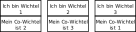
\includegraphics{images/wichtelkarten.svg}
\end{center}
enthalten.

\begin{tabular}{|l|l|}
  \hline
  \textbf{Nummer} & \textbf{Name}\\\hline
  $1$ & Carl \\\hline
  $2$ & Maryam \\\hline
  $3$ & Bertrand \\\hline
  $\vdots$ & $\vdots$\\\hline
  $n$ & Emmy\\\hline
\end{tabular}

Allgemein können wir diese Methode für $n$ Mitspieler folgendermaßen
zusammenfassen:
\begin{enumerate}
\item Wir suchen uns alle fixpunktfreien Permutationen von
  $\{1,\ldots,n\}$ heraus.
\item Für jede dieser Permutationen σ\sigmaσ bereiten wir ein Set aus
  nnn Zetteln oder Karten vor:
  \begin{enumerate}
  \item Die obere Hälfte jeder Karte wird mit einer der Zahlen aus
    $\{1,\ldots,n\}$ beschriftet.
  \item $k\in\{1,\ldots,n\}$ wird auf die untere Hälfte der mit kkk beschrifteten Karte der Wert $\sigma(k)$ geschrieben.
  \end{enumerate}
\item Jedes Kartenset stecken wir jeweils in einen anonymen
  Briefumschlag.
\item Aus den Briefumschlägen wird zufällig einer gezogen. Die übrigen
  werden versteckt oder vernichtet.
\item Jeder Mitspieler zieht eine Karte aus dem Briefumschlag (die
  niemand sonst sehen darf).
\item Es wird eine für alle sichtbare Zuordnung „Zahl
  $\leftrightarrow$ Person“ erstellt, z.B. in Form einer Tabelle:
  \begin{enumerate}
  \item Die linke Spalte enthält die Zahlen von $1$ bis $n$.
  \item In die rechte Spalte werden Namen eingetragen: Die Person, die
    auf der oberen Hälfte ihrer Karte die Zahl $k$ stehen hat,
    schreibt ihren Namen in der Tabelle in die Zeile $k$.
  \end{enumerate}
\item Jede Person schaut in der Tabelle nach, wer ihr Co-Wichtel ist:
  Person $k$ (deren Karte auf der oberen Hälfte mit kkk beschriftet
  ist), schaut auf die untere Hälfte ihrer Karte, sieht dort die Zahl
  $\sigma(k)$ ihres Co-Wichtels und findet durch einen Blick auf die
  Tabelle heraus, welche Person das ist.
\end{enumerate}

% Spoiler Wozu genau dient die Zuordnung mit Zahlen

Wir wollen dieses Vorgehen die \emph{Briefumschlag-Methode}
nennen. Sie tut genau, was wir uns wünschen: Es ist nur eine Ziehung
notwendig und jede Person kennt nur ihren Co-Wichtel und hat sonst
keine Informationen darüber, wer wem etwas schenkt. Die Sache hat nur
einen Haken: Es müssen viele Umschläge und Karten vorbereitet werden.

Erinnern wir uns, dass es bei $n$ Mitspielern $d_n =
n!\sum_{k=0}^n\frac{(-1)^k}{k!}$ fixpunktfreie Permutationen gibt. Für
jede Permutation muss ein Umschlag vorbereitet werden, der jeweils nnn
beschriftete Karten enthält. Die Fakultät in der Formel deutet es
schon an: Die Zahlen dnd_ndn​ werden für wachsende Teilnehmerzahl $n$
sehr schnell sehr groß:

\begin{tabular}{|l|l|l|}
  \hline
  $n$ & \textbf{Anzahl Umschläge $d_n$} & \textbf{Anzahl zu
                                          beschriftender Karten
                                          $n\cdot d_n$}\\\hline
  $3$ & $2$ & $6$\\\hline
  $4$ & $9$ & $36$\\\hline
  $5$ & $44$ & $220$ \\\hline
  $6$ & $265$ & $1.590$\\\hline
  $7$ & $1.854$ & $12.978$ \\\hline
  $8$ & $14.833$ & $118.664$\\\hline
  $9$ & $133.496$ & $1.201.464$\\\hline
  $10$ & $1.334.961$ & $13.349.610$\\\hline
\end{tabular}

Schon bei sechs Mitspielern muss man somit $265$ Umschläge mit jeweils
$6$ Karten vorbereiten und insgesamt $1590$ Karten beschriften! Die
Briefumschlag-Methode ist somit leider nicht wirklich
praktikabel. Aber vielleicht können wir sie modifizieren, um die
Anzahl der benötigten Umschläge und Karten zu verringern? Dafür wollen
wir das Problem aus einem etwas anderen Blickwinkel betrachten.

\section{Ändern der Fragestellung}
Bei der vorherigen Methode haben wir jede fixpunktfreie Permutation in
Form eines Umschlags angefertigt und dann aus allen Umschlägen einen
gezogen. Aber vielleicht können wir es vermeiden, alle fixpunktfreien
Permutationen erzeugen zu müssen. Dafür wollen wir das Problem anders
betrachten und zunächst überlegen, welche Eigenschaften unsere Methode
für das Wichteln eigentlich erfüllen soll.

Wir wissen schon, dass wir auf irgendeine Weise eine fixpunktfreie
Permutation $\sigma$ auf der Menge $\{1,\ldots,n\}$ der Teilnehmer
generieren müssen. Dabei soll niemand sich selbst beschenken, also
soll $\sigma$ fixpunktfrei sein. Und natürlich sollte die Methode
jeder Person $k$ ihren Co-Wichtel $\sigma(k)$ mitteilen.

Außerdem darf niemand Informationen darüber haben, wer ihn
beschenkt. Also soll die Wahrscheinlichkeit, von einer bestimmten
anderen Person beschenkt zu werden, für alle Personen gleich groß
sein. Anders gesagt: Wenn Person $k$ weiß, dass ihr Co-Wichtel Person
$k'$ ist, dann soll die Wahrscheinlichkeit, dass $k$ von irgendeinem
ihrer $n-1$ Mitspieler beschenkt wird, für jeden Mitspieler $l$ gleich
groß sein. Mathematisch ausgedrückt ist das eine bedingte
Wahrscheinlichkeit: Gegeben $\sigma(k)=k'$ soll die Wahrscheinlichkeit
für $\sigma(l)=k$ gleich $\frac{1}{n-1}$ für alle $l\ne k$ sein. In Formeln:

\[
  P(\sigma(l)=k\mid\sigma(k)=k')=\frac{1}{n-1}\quad\text{für alle}\quad l\neq k.
\]

Bei der Briefumschlag-Methode wird die zweite Eigenschaft mit den
Wahrscheinlichkeiten dadurch erfüllt, dass wir aus allen
fixpunktfreien Permutationen losen. Leider sind das so viele, dass wir
die ganzen Umschläge nicht mehr erstellen können.

Wir können das Problem aber auch andersherum angehen. Anstatt alle
fixpunktfreien Permutationen zu erzeugen, starten wir mit nur einer
fixpunktfreien Permutation $\sigma$. Diese ist allen bekannt. Dann
brauchen wir minimal viele Umschläge, und zwar keinen, da wir nur eine
Permutation haben und keine mehr auszulosen brauchen. Weil aber jeder
die Permutation kennt, sind wir maximal weit von unserem Ziel
entfernt, dass niemand Informationen darüber hat, wer wen beschenkt.

Wie können wir davon ausgehend die Permutation $\sigmaσ$ zufälliger
machen?

\section{Die Konjugations-Methode}
Angenommen wir haben eine fixpunktfreie Permutation $\sigma\colon
\{1,\ldots,n\}\to\{1,\ldots,n\}$ gegeben, ordnen jedem Mitspieler eine
der Zahlen von $1$ bis $n$ zu und benutzen $\sigma$ zum Wichteln. Das
heißt, Person $k$ soll der Wichtel von Person $\sigma(k)$ sein. Wenn
nun ein Teilnehmer die ganze Permutation $\sigma$ kennt, kann er ihre
Inverse $\sigma^{-1}$ (die Umkehrfunktion von $\sigma$) bestimmen und
damit herausfinden, wer sein Wichtel ist. Deshalb können wir nicht
einfach allen Teilnehmern ihre Nummer und die Permutation $\sigma$
mitteilen, sondern müssen die Zuordnung „zufälliger“ gestalten, indem
wir eine der Informationen unbekannt machen.

Die Permutation $\sigma$ zu kennen kann den Mitspielern nur dann etwas
über ihre (Co-)Wichtel verraten, wenn alle wissen, wem welche Zahl
zugeordnet ist. Ohne diese Information ist es für eine Person nicht
möglich, ihren Wichtel oder Co-Wichtel herauszufinden. Damit können
wir etwas über die Zuordnung von Wichteln zu Co-Wichteln unbekannt
machen: Wir wollen eine Methode finden, um jeder Person $k$ ihren
Co-Wichtel $\sigma(k)$ zuzuordnen, ohne dass bekannt wird, welcher
Person welche Nummer zugeordnet war. Wie können wir das anstellen?

Eine Möglichkeit wäre, die Personen $\{1, \dots, n\}$ zunächst
durchzumischen, also alle Teilnehmer auf zufällige Art und Weise
„umzubenennen“, indem wir ihnen neue Zahlen $\{1,\ldots,n\}$
zuweisen. Dann wenden wir $\sigma$ auf diese neue Reihenfolge an.

\begin{center}
  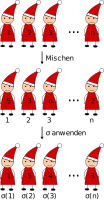
\includegraphics{images/wichtelmischen.svg}
\end{center}

Weil $\sigma$ bekannt ist, kann man zwar immer noch $\sigma^{-1}$
berechnen, aber man weiß nicht mehr, zu welcher Person die Zahl
$\sigma^{-1}(k)$ gehört. Damit haben wir die Zuordnung von Wichteln zu
Co-Wichteln zufälliger gemacht. Die Frage ist nun, wie wir das
praktisch durchführen können.

Wir betrachten jeden Wichtel als eine Karte. Diese Karten drehen wir
um, mischen sie und bringen sie (immer noch verdeckt) in eine
Reihenfolge. Nun möchten wir auf diese neue verdeckte Reihenfolge die
Permutation $\sigma$ anwenden. Wir können nicht einfach die Karten neu
anordnen, da wir so vergessen, zu welchem Wichtel der ursprüngliche
Platz gehört.

Wenn wir die Information, welcher Wichtel auf der Karte ist, zweimal
schreiben, können wir die Karten nach dem Mischen durchschneiden und
$\sigma$ auf eine Hälfte der Karten anwenden (zum Beispiel die obere
Hälfte jeder Karte).

\begin{center}
  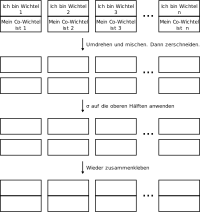
\includegraphics{images/wichtelkartenmischen.svg}
\end{center}

Nun müssen wir die Karten nur wieder dem echten Wichteln $\{1, \dots,
n\}$ zuordnen, damit jeder Wichtel seinen Co-Wichtel erfährt. Das
können wir in der Praxis nun ganz einfach machen: (Unsere Wichtel
heißen ja in der Realität anders als $1, \dots, n$.) Wir kleben die
neu sortierten Karten wieder zusammen, schmeißen sie in einen Hut und
jeder zieht sich eine Karte. Auf jeder Karte steht nun, welche Zahl
$1, \dots, n$ er selbst ist und welche Zahl $1, \dots, n$ sein
Co-Wichtel ist. Wir müssen damit nur noch eine Liste anlegen, auf der
steht, welche Zahl zu welcher Person korrespondiert.

\begin{tabular}{|l|l|}
  \hline
  \textbf{Nummer} & \textbf{Name}\\\hline
  $1$ & Julia\\\hline
  $2$ & Kurt\\\hline
  $3$ & Katherine \\\hline
  $\vdots$ & $\vdots$\\\hline
  $n$ & David \\\hline
\end{tabular}

Diesen Vorgang bezeichnen wir als \emph{Konjugations-Methode}.

% Spoier, was passiert hier mathematisch

\section{Erste Ansätze mit der Konjugations-Methode}
Um die Konjugationsmethode zu verwenden, benötigen wir eine
fixpunktfreie Permutation $\sigma$. Eine einfache fixpunktfreie
Permutation ist die Abbildung, welche die Elemente von
$\{1,\ldots,n\}$ „zyklisch“ um eine Position verschiebt, d.h. die
Abbildung $\sigma\colon \{1, \dots, n\} \to \{1, \dots, n\}$, die der
Tabelle
\[
  \begin{bmatrix} 1 & 2 & 3 & \cdots & n-1 & n\\ 2 & 3 & 4 & \cdots & n & 1 \end{bmatrix}
\]
entspricht.

\begin{center}
  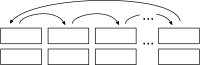
\includegraphics{images/zyklischepermutation.svg}
\end{center}

Erinnern wir uns an das Ziel, das wir mit unserer Wichtelmethode
erreichen wollen: Wir wollen, dass die bedingte Wahrscheinlichkeit
$P(\sigma'(i)=k\mid\sigma'(k)=k')=\frac{1}{n-1}$ für jedes $i \ne k$
ist. Mit anderen Worten, die Wahrscheinlichkeit, dass man von einem
gewissen Mitspieler beschenkt wird, soll für alle Mitspieler gleich
groß sein, gegeben, dass man weiß, wer der eigene Co-Wichtel
ist. Haben wir dieses Ziel erreicht, wenn wir $\sigma$ mit der
Konjugationsmethode zu einer Permutation $\sigma'$ zufällig ändern?

Wenn wir $\sigma$ auf eine Karte $k$ anwenden und die Karte $k'$
erhalten, kann $k'$ durch $\sigma$ nicht auf $k$ geschickt
werden. Zumindest, wenn wir mit mindestens $3$ Karten arbeiten. Damit
ist für $n \ge 3$ die Wahrscheinlichkeit
$P(\sigma'(k')=k\mid\sigma'(k)=k')=0$ und $k'$ nie der Wichtel von
$k$. Weil wir mischen, kann aber jede andere Person, die nicht $k$
oder $k'$ entspricht, der Wichtel von $k$ sein. Von diesen gibt es
$n-2$ viele. Wir erhalten also
\[
  P(\sigma'(i) = k\mid \sigma'(k) = k') = \begin{cases} \frac{1}{n-2}, & \text{falls }i \ne k'\\ 0, & \text{falls }i = k'. \end{cases}.
\]
Damit stimmen die Wahrscheinlichkeiten nicht mit den gewünschten
überein: Die Wahrscheinlichkeit, dass man von einer bestimmten anderen
Person beschenkt wird, ist mit $0$ zu klein, wenn man ihr Wichtel ist,
und mit $\frac{1}{n-2}$ zu groß, wenn man nicht ihr Wichtel ist.

\subsection{Eine andere Permutation}
Wenn die Wahrscheinlichkeit, jemandes Co-Wichtel zu sein, für alle
Personen (außer einem selbst) gleich sein soll, müssen wir also eine
andere Permutation ausprobieren. Das Problem ist, dass $\sigma$ es
nicht zulässt, von seinem eigenen Co-Wichtel als Co-Wichtel gezogen zu
werden. Wir benötigen also eine Permutation, auf die das zutrifft. Was
muss eine solche Permutation $\varphi$ erfüllen? Es soll eine Person
$i$ geben, deren Co-Wichtel $\varphi(i)$ der Wichtel von $i$ selbst
ist. Es soll also ein $i$ geben, sodass $\varphi(\varphi(i)) = i$
gilt.

Eine einfache solche Permutation $\varphi\colon\{1,\dots, n\} \to
\{1,\dots, n\}$ können wir für $n \ge 4$ durch die folgende Tabelle
bauen:
\[
  \begin{bmatrix} 1 & 2 & 3 & 4 & \cdots & n-1 & n\\ 2 & 1 & 4 & 5 & \cdots & n & 3 \end{bmatrix}.
\]

\begin{center}
  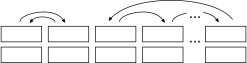
\includegraphics{images/nichtzyklischepermutation.svg}
\end{center}

Wie sehen die Wahrscheinlichkeiten für diese Permutation aus? Wir
haben durch die Konjugationsmethode mit $\varphi$ eine Permutation
$\varphi'$ erhalten und diese hat $\varphi'(k) = k'$. Wenn die Karte
$k$ beim Mischen zur ersten oder zweiten Karte wird, ist der Wichtel
von $k$ sicher $k'$. Dies passiert mit der Wahrscheinlichkeit $\frac
2n$. Wenn $k$ beim Mischen zu irgendeiner anderen Karte wird, ist $k'$
nie der Wichtel von $k$. Somit haben wir $P(\varphi'(k') = k\mid
\varphi'(k) = k') = \frac 2n$. Im anderen Fall, wo $k$ durchmischen
nicht zur ersten oder zweiten Karte wird, ist jeder andere Person, die
nicht $k$ oder $k'$ ist, als Wichtel gleich wahrscheinlich. Das sind
noch $n-2$ Personen. Diese müssen sich die Restwahrscheinlichkeit
damit gleichmäßig aufteilen und wir erhalten $P(\varphi'(i) = k \mid
\varphi'(k) = k') = (1-\frac 2n) \cdot \frac{1}{n-2} = \frac
1n$. Zusammengefasst hat $\varphi'$ die Wahrscheinlichkeiten
\[
  P(\varphi'(i) = k\mid \varphi'(k) = k') = \begin{cases} \frac{1}{n}, & \text{falls }i \ne k'\\ \frac{2}{n}, & \text{falls }i = k'. \end{cases}.
\]
Hier ist die Wahrscheinlichkeit, dass man der Co-Wichtel seines
Co-Wichtels ist, mit $\frac{2}{n}$ zu hoch, und die
Wahrscheinlichkeit, jemand anderes als Wichtel zu haben, mit
$\frac{1}{n}$ zu gering. Für unsere Rechnung müssen wir auf ein Detail
aufpassen: Sie funktioniert nur, wenn $n \ge 5$.

% Spoiler, Warum funktioniert die Rechnung nur für $n \ge 5$?

Wir haben jetzt eine Permutation gefunden, bei der die
Wahrscheinlichkeiten jeweils zu hoch und eine, wo sie jeweils zu
niedrig sind. Können wir dies kombinieren, sodass die
Wahrscheinlichkeiten passen?

\section{Die verbesserte Konjugations-Methode}
Wir haben zwei Ausgangspermutationen σ\sigmaσ und φ\varphiφ gefunden. Bei einer
ist die Wahrscheinlichkeit zu klein, dass man der Co-Wichtel seines Co-Wichtels
ist, und bei der anderen zu groß. Um dieses Problem zu beheben, wollen wir beide
Permutationen kombinieren, um die korrekten Wahrscheinlichkeiten zu
erhalten. Wir wollen also mit einer gewissen, noch zu bestimmenden
Wahrscheinlichkeit ppp die Konjugations-Methode mit σ\sigmaσ anwenden und mit
Wahrscheinlichkeit 1−p1-p1−p die Konjugations-Methode mit φ\varphiφ anwenden.

% Spoiler Warum suchen wir nicht einfach eine dritte Permutation, die die
% korrekten Wahrscheinlichkeiten liefert?

Wie müsste die Wahrscheinlichkeit $p$ sein, damit die Wahrscheinlichkeit, der
Co-Wichtel seines Co-Wichtels zu sein, genau $\frac{1}{n-1}$ ist? Bei $\sigma$
ist die Wahrscheinlichkeit null und bei $\varphi$ ist die Wahrscheinlichkeit
$\frac 2n$. Wir wollen also, dass $\frac{1}{n-1} = 0\cdot p + (1-p)\cdot
\frac{2}{n}$. Damit können wir $p$ berechnen:

\begin{align*}
  (1-p)\cdot\frac{2}{n} & = \frac{1}{n-1} & \mid \cdot \frac n2\\
  1-p & = \frac{n}{2(n-1)} & \mid -1\\
  -p & \frac{n\ -\ 2n\ +\ 2}{2\left(n-1\right)} & \mid \cdot (-1)\\
  p & \frac{n-2}{2n-2} & 
\end{align*}

Das heißt, wir müssen mit der Wahrscheinlichkeit $\frac{n-2}{2n-2}$ die
Konjugations-Methode mit $\varphi$ anwenden und mit Wahrscheinlichkeit
$\frac{n}{2n-2}$ mit $\sigma$.

Wenn unsere Methode funktioniert, müssen die anderen Wahrscheinlichkeiten
ebenfalls passen: Bei $\sigma$ ist die Wahrscheinlichkeit, dass eine Person
einen selbst als Co-Wichtel hat, die nicht der Co-Wichtel von einem ist, genau
$\frac{1}{n-2}$. Bei $\varphi$ ist diese Wahrscheinlichkeit $\frac{1}{n}$. Somit
haben wir bei unserer Kombination die Wahrscheinlichkeit $p\cdot \frac{1}{n-2} +
(1-p)\cdot \frac 1n = \frac{1}{n-1}$. Das heißt, diese Mischung liefert eine
geheime Wichtelzuordnung.

Wir haben schon einmal gesehen, wie wir eine Permutation zufällig ziehen können,
ohne zu wissen, welche wir gezogen haben: Mit der Briefumschlag-Methode. Wir
können also versuchen, unser Problem mit dieser zu lösen. Dafür benötigen wir
genug Umschläge, damit das Wahrscheinlichkeitsverhältnis stimmt.

Damit dieses Verhältnis stimmt, müssen wir $n$ Versionen von $\sigma$ haben und
$n-2$ Versionen von $\varphi$. In den Umschlägen können aber nicht immer die
gleichen Permutationen $\sigma$ bzw. $\varphi$ liegen, da wir auf diese dann
erst die Konjugations-Methode anwenden müssten und wir dafür die gezogene
Permutation aufdecken müssten. Damit müssen die Permutationen, die wir in die
Umschläge gesteckt haben, schon aus der Konjugations-Methode stammen.

Wir machen also folgendes:
\begin{enumerate}
\item Wir präparieren nnn Briefumschläge mit der Konjugations-Methode mit
  $\sigma$ und $n-2$ Briefumschläge mit der Konjugations-Methode mit $\varphi$.
\item Wir werfen alle Umschläge in einen Hut (oder Ähnliches), mischen und
  ziehen einen Umschlag.
\item Die Karten dieses Umschlags werden nun wie bei der Briefumschlag-Methode
  ausgeteilt und verwendet.
\end{enumerate}

Da diese Methode die Konjugations-Methode verbessert, werden wir sie die
\emph{verbesserte Konjugations-Methode} nennen.

Damit haben wir eine Methode gefunden, wie wir mathematisch korrekt wichteln
können. Es stellt sich nur die Frage, wie viele Karten wir erstellen müssen:
Wenn wir $2n-2$ Briefumschläge erstellen müssen und jeder Umschlag $n$ Karten
enthält, müssen wir $n\cdot (2n-2)$ Karten erstellen und die
Konjugations-Methode $2n-2$ Mal anwenden. Dies werden ziemlich schnell ziemlich
viele Karten:

\begin{tabular}{|l|l|l|}
  \hline
  \textbf{Teilnehmer} & \textbf{Anzahl Umschläge} & \textbf{Anzahl
                                                    Zettel}\\\hline
  \hline
  5 & 8 & 40\\\hline
  7 & 12 & 84\\\hline
  10 & 18 & 180 \\\hline
  25 & 48 & 1200 \\\hline
\end{tabular}

Lohnt sich diese Methode trotzdem, bzw. können wir sie praktikabel machen?

\section{Wie können wir unsere Methode praktikabler machen?}
\subsection{Sehr viel Arbeit für eine Person}
Wenn $n$ Personen wichteln, brauchen wir mit der verbesserten
Konjugations-Methode $2n-2$ Umschläge und in jedem Umschlag $n$ Karten. Also
muss man insgesamt $n\cdot (2n-2)$ Karten schreiben.

Wir könnten die Karten am Computer erstellen und entsprechend oft
drucken. Dadurch sparen wir uns das Beschriften der $n\cdot(2n-2)$ Karten und
wir müssen diese Karten nur ausschneiden. Jedoch müssen wir für jeden Umschlag
die entsprechende Permutation $\sigma$ oder $\varphi$ anwenden und mit einer
Permutation konjugieren. Die Permutationen $\sigma$ und $\varphi$ sind gegeben
durch
\[
  \begin{bmatrix} 1 & 2 & 3 & \cdots & n-1 & n\\ 2 & 3 & 4 & \cdots & n & 1 \end{bmatrix}
\]
und
\[
  \begin{bmatrix} 1 & 2 & 3 & 4 & \cdots & n-1 & n\\ 2 & 1 & 4 & 5 & \cdots & n & 3 \end{bmatrix}.
\]
Konkret heißt das, wir mischen die Karten, schneiden sie auseinander,
verschieben die Hälfte entsprechend der Permutation $\sigma$ oder $\varphi$ und
kleben sie wieder zusammen.

Das ist immer noch viel Arbeit für eine Person.

Die Anzahl der Umschläge steigt linear mit der Anzahl der Personen. Deshalb wird
es immer mehr Arbeit, je mehr Personen mitwichteln. Aber wir können die Arbeit
auf alle Personen aufteilen: Jede Person erstellt zwei Umschläge, einen mit der
Permutation $\sigma$ und einen mit der Permutation $\varphi$. Dann haben wir $n$
Umschläge je Permutation $\sigma$ und $\varphi$. Für das richtige Verhältnis
brauchen wir aber $n-2$ Umschläge mit $\varphi$, also müssen wir $2$ Umschläge
mit der Permutation $\varphi$ aussortieren. Wenn wir die Karten drucken, kann
man durch die Handschrift nicht die Person erkennen. Dann müssen zwei Leute nur
einen Umschlag mit der Permutation $\sigma$ erstellen.

Dadurch muss, egal wie viele Leute mitwichteln, jede Person höchstens $2$
Umschläge anfertigen. Leider steigt die Anzahl der Karten, die jeder
ausschneiden muss, mit $n$. Also muss jeder $n$ oder $2n$ Karten vorbereiten.

\subsection{Wiederverwenden der Umschläge}
Neben dem hohen Aufwand hat die verbesserte Konjugations-Methode noch einen
Nachteil: Weil wir nur einen Umschlag ziehen, haben wir sehr viele Umschläge und
Karten, die nicht verwendet werden. Wir können sie auch nicht so einfach
wiederverwenden. Denn wenn wir die unbenutzten Umschläge öffnen, würden wir
herausfinden, welcher Umschlag für das Wichteln benutzt wurde. Wir müssten die
ungeöffneten Umschläge also vernichten, was nicht sehr nachhaltig ist.

Wir können diesen Müll aber doch vermeiden: Wir sammeln alle Karten von dem
benutzten Umschlag wieder ein, legen sie zurück in den Umschlag und verschließen
diesen so, dass man ihn nicht von den anderen, unbenutzten unterscheiden
kann. Dann kann man die Umschläge im nächsten Jahr wiederverwenden. Das geht
aber nur, wenn wieder gleich viele Personen beim Wichteln mitmachen. Wenn mehr
oder weniger mitwichteln, müssen wieder ganz neue Umschläge gebastelt werden.

\section{Zusammenfassung}
Wir haben verschiedene Methoden kennengelernt, die man zum Wichteln mit nnn
Teilnehmern benutzen kann.

Zum einen gibt es die klassische Wichtel-Methode. Dabei werden Zettel mit Namen
aus einem Hut gezogen und so eine geheime Zuordnung von Wichteln (Schenkenden)
zu Co-Wichteln (Beschenkten) erstellt. Mathematisch kann man eine solche
Zuordnung als eine Permutation auf $\{1,\ldots,n\}$ auffassen. Der Nachteil
dieser Methode ist, dass die durch das Ziehen der Zettel erzeugte Permutation
möglicherweise nicht fixpunktfrei ist, also Personen ihren eigenen Namen ziehen
können. Dann muss man die Ziehung wiederholen. Im Schnitt braucht man etwa drei
Versuche.

Deshalb haben wir versucht, eine Methode zu finden, bei der man garantiert mit
einer Ziehung auskommt. Unser erster Ansatz war die Briefumschlag-Methode. Dabei
wählen wir statt aus allen Permutationen nur aus den fixpunktfreien
Permutationen. Um die Zuordnung geheim zu halten, war es nötig, für jede
fixpunktfreie Permutation einen Umschlag mit nnn Karten zu erstellen, von denen
einer ausgelost wird. Da aber die Anzahl der fixpunktfreien Permutationen mit
steigender Teilnehmerzahl sehr schnell wächst, ist diese Methode nicht
praktikabel - bei zehn Teilnehmern müsste man über eine Million Umschläge
vorbereiten!

Eine andere Methode musste her. Dafür haben wir das Problem aus einem anderen
Blickwinkel betrachtet und uns zuerst unsere Anforderungen an eine
Wichtel-Methode vergegenwärtigt: Für jede Person soll, unter der Annahme, dass
sie ihren Co-Wichtel kennt, die Wahrscheinlichkeit, von einem ihrer Mitspieler
beschenkt zu werden, für jeden Mitspieler gleich groß sein. Bei der
Briefumschlag-Methode haben wir das Problem durch schiere Masse erschlagen.

Die Konjugations-Methode dagegen startet mit einer festen fixpunktfreien
Permutation und macht diese "zufälliger", indem die Zuordnung von Teilnehmern zu
den Zahlen $\{1,\ldots,n\}$ durchmischt wird. Wir haben uns diese Methode für
zwei fixpunktfreie Permutationen $\sigma$ und $\varphi$ angeschaut. Je nachdem,
von welcher Permutation man ausgeht, ist jedoch die Wahrscheinlichkeit, vom
eigenen Co-Wichtel beschenkt zu werden, entweder zu hoch oder zu niedrig.

Um den Wert $\frac{1}{n-1}$ zu erreichen, muss man die beiden Permutationen
kombinieren und mit der passenden Wahrscheinlichkeit entweder $\sigma$ oder
$\varphi$ beim Wichteln mit der Konjugations-Methode verwenden. Die Methode, die
das tut, haben wir die verbesserte Konjugations-Methode genannt. Sie kombiniert
die Konjugations- mit der Briefumschlag-Methode und ist unser bester Kandidat
für eine Wichtel-Methode, bei der garantiert nur einmal gezogen werden muss:

\begin{enumerate}
\item Wir präparieren nnn Briefumschläge mit der Konjugations-Methode mit $\sigma$ und
$n-2$ Briefumschläge mit der Konjugations-Methode mit $\varphi$.
\item Wir werfen alle Umschläge in einen Hut (oder Ähnliches), mischen und
  ziehen einen Umschlag.
\item Die Karten dieses Umschlags werden nun wie bei der Briefumschlag-Methode ausgeteilt und verwendet.
\end{enumerate}

Man braucht also bei $n$ Mitspielern nur $2n-2$ Umschläge. Diese Menge ist gut
zu bewältigen, wenn man die Arbeit auf die Teilnehmer aufteilt und jeden zwei
Umschläge (einen mit $\sigma$ und einen mit $\varphi$) vorbereiten lässt.

Wer hätte gedacht, dass mit so etwas Alltäglichem so viel interessante
Mathematik treiben kann. Und wer würde jetzt noch behaupten, dass Mathematik
nicht lebensnah ist!

%%% Local Variables:
%%% mode: LaTeX
%%% TeX-master: "../../mfnf"
%%% End:
